\chapter{Cơ học}
\section{Động học chất điểm}
\subsection{Chuyển động thẳng đều}
\begin{center}
    $s=vt$\\
    $x=x_{0}+vt$\\
\end{center}
\subsection{Chuyển động thẳng biến đổi đều}
\subsubsection{Công thức}
Dưới đây là các công thức đều đã được học ở THPT, tất cả các công thức này đều cần thuộc kĩ:
\begin{tcolorbox}
    $$v=v_{0}+at$$
    $$x=x_{0}+v_{0}t+\frac{1}{2}at^2$$
    $$v^2-v_{0}^2=2as$$
    $$s=v_{0}t+\frac{1}{2}at^2$$
\end{tcolorbox}
\subsubsection{Bài toán ném xiên và ném ngang}
1. Cho một vật bị ném ngang tại gốc tọa độ $O$ ở độ cao $h$ so với mặt đất với vận tốc ban đầu $v_{O}$, hãy khảo sát chuyển động của vật.\\
\begin{figure}
    \centering
    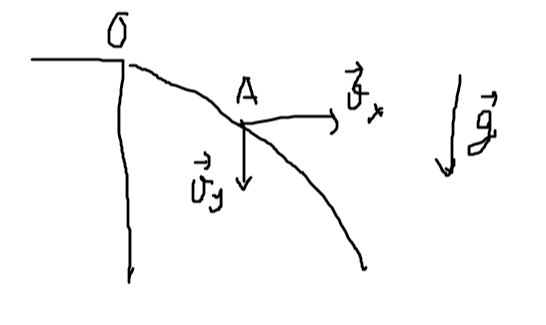
\includegraphics[width=0.5\textwidth]{nem_ngang.png}
    \caption{Chuyển động ném ngang}
    \label{nem_ngang}
    \end{figure}
Chọn hệ trục tọa độ $Oxy$ với trục $Ox$ hướng sang phải và trục $Oy$ hướng cùng chiều với chiều của gia tốc trọng trường.
Do chuyển động theo phương $Ox$ là chuyển động thẳng đều, còn chuyển động theo phương $Oy$ là chuyển động thẳng biến đổi đều, ta suy ra:
    $$\left\{\begin{array}{ll}
    v_{x}=v_{O} &\\
    v_{y}=gt &\\
    \end{array}\right.$$
Ta tiếp tục suy ra được công thức xác định tọa độ vật đi được theo 2 phương:
$$\left\{\begin{array}{ll}
    x=v_{O}t&\\
    y=\frac{1}{2}gt^2 &\\
\end{array}\right.$$
Ta suy ra được phương trình chuyển động của vật:
\begin{equation}
    y=\frac{gx^2}{2v_{O}^2}
\end{equation}
Ta xác định được tầm ném xa $L$ của vật khi ném ở độ cao $h$ là:
\begin{equation}
    L=v_{O}\sqrt{\frac{2h}{g}}
\end{equation}
Thời gian $T$ tính từ lúc ném cho đến khi vật chạm dất là:
\begin{equation}
    T=\sqrt{\frac{2h}{g}}
\end{equation}
\newpage
2. Cho một vật bị ném xiên với góc ném $\alpha$ tại gốc tọa độ $O$ trên mặt đất với vận tốc đầu $v_{O}$, khảo sát chuyển động của vật.\\
\begin{figure}
    \centering
    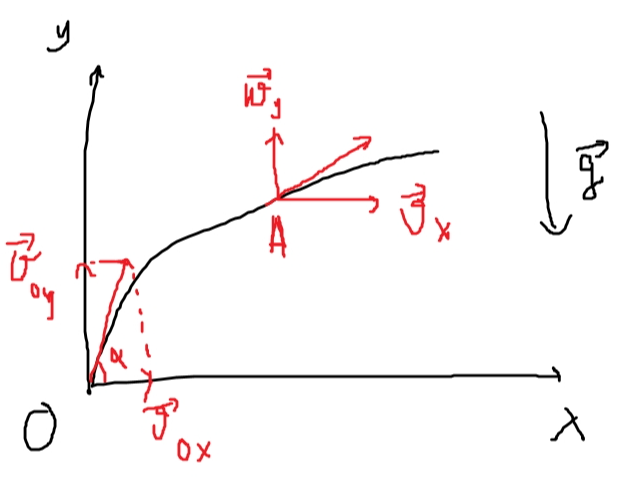
\includegraphics[width=0.5\textwidth]{nem_xien.png}
    \caption{Chuyển động ném xiên}
    \label{nem_xien}
\end{figure}
\textbf{Lưu ý khi vẽ hình:} Vector vận tốc $\vec{v}$ tại một điểm bất kì luôn trùng phương với phương của tiếp tuyến tại điểm đó\\
Chọn chiều dương với chiều của trục $Ox$ hướng từ trái sang phải và chiều của trục $Oy$ ngược với chiều của gia tốc trọng trường\\
Xét vật tại gốc tọa độ $O$, ta thấy:
$$\left\{\begin{array}{ll}
    v_{Ox}=v_{O}\cos{\alpha}&\\
    v_{Oy}=v_{O}\sin{\alpha}&\\
\end{array}\right.$$
Tại một điểm A bất kì trên phương chuyển động, ta nhận thấy chuyển động theo phương $Ox$ là chuyển động thẳng đều còn chuyển động theo phương $Oy$ là chuyển động thẳng biến đổi đều với gia tốc $g$. Ta dễ dàng suy ra được:
$$\left\{\begin{array}{ll}
    v_{Ax}=v_{O}\cos{\alpha}&\\
    v_{Ay}=v_{O}\sin{\alpha}-gt&\\
\end{array}\right.$$
Ta suy ra tọa độ của điểm A:
$$\left\{\begin{array}{ll}
    x=v_{O}\cos{\alpha}t&\\
    y=v_{O}\sin{\alpha}t-\frac{g}{2}t^2&\\
\end{array}\right.$$
Ta thế biến $t$ của 2 phương trình trên với nhau và tìm ra được phương trình chuyển động của vật:
\begin{equation}
    y=x\tan{\alpha}-\frac{g}{2v_{O}^2\cos{\alpha}^2}x^2
\end{equation}
Tiếp theo ta sẽ xác định tầm xa cực đại $L_{max}$ và độ cao cực đại $H_{max}$ của vật
Khi vật chạm đất, ta thấy:
$$y=0$$
$$\Rightarrow x\tan{\alpha}-\frac{g}{2v_{O}^2\cos^2{\alpha}}x^2=0$$
$$\Rightarrow L=\frac{v_{O}^2}{g}\sin{2\alpha}$$
Để $L$ max thì $\sin{2\alpha}=1$, tương đương với $\alpha=\frac{\pi}{4}$\\
Tại điểm vật đạt độ cao cực đại $H_{max}$ thì $v_{y}=0$, ta suy ra được:
$$t=\frac{v_{O}\sin{\alpha}}{g}$$
\begin{equation}
    \Rightarrow H_{max}=\frac{v_{O}^2.\sin^2{\alpha}}{2g}\leq \frac{v_{O}^2}{2g}
\end{equation}
Bài tập:
\begin{enumerate}
    \item Xây dựng lại công thức ném xiên và ném ngang.
    \item Hai vật được ném đi từ cùng 1 điểm, vật thứ nhất được ném lên thẳng đứng với vận tốc $v_{0}=25m/s$, vật thứ 2 được ném từ cùng một địa điểm với cùng vận tốc đầu theo phương ngang với góc 60 độ. Xác định khoảng cách giữa hai vật sau khoảng thời gian 1.7s. (Đáp án: 22m)
\end{enumerate}
\subsection{Chuyển động tròn đều}
Chuyển động tròn đều là một trường hợp tương đối "đặc biệt" vì mặc dù độ lớn của vận tốc không đổi nhưng hướng của nó luôn thay đổi, vì thế nên chuyển động tròn đều tồn tại gia tốc hướng tâm có độ lớn:
$$a=\frac{v^2}{r}$$
\newpage
\section{Động lực học chất điểm}
\subsection{3 định luật Newton}
\begin{tcolorbox}
    \begin{enumerate}
        \item Một vật đứng yên hay chuyển động thẳng đều nếu vật đó không bị lực nào tác dụng.
        \item Tổng vector các lực tác dụng lên chất điểm bằng khối lượng của chất điểm nhân gia tốc mà nó nhận được dưới tác dụng của các lực đó.
        $$\sum \vec{F}=m\vec{a}$$
        \item Phản lực luôn luôn bằng và ngược hướng với lực tác dụng
        $$\vec{F_{12}}=-\vec{F_{21}}$$ 
    \end{enumerate}
\end{tcolorbox}
\subsection{Lực ma sát}
Lực ma sát là lực rất \textbf{thường xuyên xuất hiện trong các bài tập} nếu đề bài không cho bỏ qua ma sát:
$$F_{ms}=N\mu$$
Lực ma sát có chiều ngược với chiều chuyển động của vật.
\subsection{Lực trong chuyển động tròn đều}
Để giữ cho một vật chuyển động tròn đều thì cần có lực hướng tâm, độ lớn lực hướng tâm được xác định theo định luật II Newton như sau:
\begin{equation}
    F_{ht}=ma_{ht}=\frac{mv^2}{r}
\end{equation}
Bài tập:
\begin{enumerate}
    \item Một người có khối lượng $m_{1}=60kg$ đứng trong thang máy $m_{2}=300kg$. Thang máy chuyển động lên trên với gia tốc $a=0.8 m/s^2$. Tính lực căng của dây cáp treo thang máy, lực người đó nén lên sàn trong hai trường hợp
    \begin{itemize}
        \item Nhanh dần đều (Đáp án: 3816; 636)
        \item Chậm dần đều (Đáp án: 3240; 540)
    \end{itemize}
    \item Một vật có khối lượng 1kg được buộc vào đầu dây có chiều dài l=30cm, một đầu của dây được giữ cố định vào gốc O. Cho vật chuyển động tròn đều trong mặt phẳng ngang, còn sợi dây hợp với phương thẳng đứng góc 60 độ. Tính vận tốc của vật và sức căng của sợi dây (Đáp án: v = 2.1m/s, T = 19.6N)
    \item Một vật A có khối lượng $m_{1}=3kg$ nằm trên mặt phẳng nghiêng góc 30 độ so với phương nằm ngang. Vật A được nối với vật B có khối lượng $m_{2}=2kg$ bằng một sợi dây không co dãn qua một ròng rọc cố định. Hãy xác định gia tốc chuyển động của các vật và lực căng của dây, biết hệ số ma sát giữa vật A và mặt phẳng nghiêng là $\mu=0.1$. (Đáp án: a = 0.47$m/s^2$, T = 18.7N)
\end{enumerate}
Gợi ý: Vẽ hình, phân tích các lực tác dụng lên vật và dùng phương trình $F=ma$\\
Đối với bài 3, đầu tiên vẽ hình ra và phân tích lực của 2 vật A và B, sau đó so sánh độ lớn giữa hai lực $F_{ms}$ của vật A và $P_{B}$ để tìm ra chiều chuyển động của cơ hệ.
\begin{figure}
    \centering
    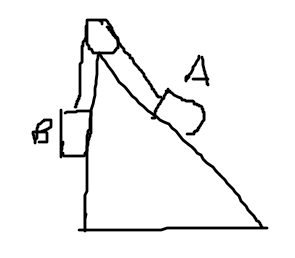
\includegraphics[width=0.3\textwidth]{co_he.png}
    \caption{Cơ hệ bài 3}
    \label{co_he}
\end{figure}
\subsection{Công và năng lượng}
\subsubsection{Công}
Ta có 2 công thức tính công trong các trường hợp:
\begin{itemize}
    \item $A=F.s.\cos{\phi}$ trong trường hợp $F$ không đổi
    \item $$A=\int_{x_{1}}^{x_{2}}F(x)dx$$ \\ trong trường hợp $F$ thay đổi và $F(x)$ là một hàm theo $x$, tức là độ lớn lực $F$ là một hàm theo ly độ x. Hãy nhớ công thức này vì nó \textbf{rất quan trọng về sau}
\end{itemize}
\subsubsection{Động năng và định lý biến thiên động năng}
Động năng là đại lượng đặc trưng cho năng lượng của vật gắn liền với chuyển động của nó. Ta có: $$W_{d}=\frac{mv^2}{2}$$
Ta có biến đổi sau:
   $$ A=\int_{x_{1}}^{x_{2}}F(x)dx=\int_{x_{1}}^{x_{2}}m.adx=\int_{t_{1}}^{t_{2}}mavdt=\int_{v_{1}}^{v_{2}}mvdv=\frac{mv_{2}^2}{2}-\frac{mv_{1}^2}{2}=\Delta W_{d}$$
Vậy biến thiên động năng của chất điểm ở trạng thái cuối và đầu bằng công A của các lực tác dụng lên vật đó.
\subsubsection{Thế năng}
Thế năng là đại lượng đặc trưng cho năng lượng của vật gắn liền với vị trí của nó. Ta xét hai loại thế năng đơn giản nhất là thế năng đàn hồi và thế năng trọng trường.\\
1. Thế năng đàn hồi: Ta xét một lò xo gắn cố định 1 đầu trên mặt phẳng ngang, theo định luật Hooke, ta xác định được lực kéo về $F$ như sau: $F(x)=-kx$
\begin{figure}
    \centering
    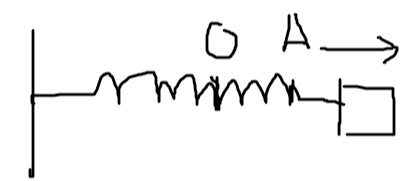
\includegraphics[width=0.5\textwidth]{lo_xo.png}
    \caption{Lò xo bị kéo ra một khoảng $\Delta l$}
    \label{lo_xo}
\end{figure}
\\Ta có thể tính được công của lò xo thực hiện được khi kéo vật từ điểm O(lò xo ở chiều dài tự nhiên) đến A (lò xo bị kéo) là:
$$A=\int_{0}^{x}F(x)dx=-\frac{1}{2}kx^2$$
Công mà lực kéo thực hiện được ngược dấu với công của lò xo thực hiện được để kéo vật trở về vị trí cân bằng
$$A'=\frac{1}{2}kx^2$$
Ta đặt $$A'=W_{t}$$ và gọi $W_{t}$ là thế năng đàn hồi (tức là năng lượng mà lò xo tích trữ được) tại điểm A.
\\
2. Thế năng trọng trường: Ta xét một vật có khối lượng m nằm cách đất một độ cao h xác định:
Tại điểm A đó, vật chịu tác dụng của trọng lực:$$P=mg$$
Khi vật rơi từ điểm A xuống đất, ta tính công của vật:
$$A=\int_{0}^{h}Pdx=mgh$$
Khi vật chạm đất, nó đã thực hiện công A, ta gọi $W_{t}$ là thế năng trọng trường của vật tại điểm A vì tại điểm đó vật lưu trữ một lượng năng lượng $W_{t}=mgh$
\subsubsection{Công suất}
Công suất là một đại lượng đặc trưng cho khả năng sinh công nhanh hay chậm:
$$P=\frac{A}{t}$$ với thứ nguyên của $P$ là $W$, $1W=1J/s$
\subsubsection{Định luật bảo toàn cơ năng}
Cơ năng được định nghĩa là tổng động năng và thế năng của một vật, hay tức là năng lượng của vật tại một thời điểm xác định nào đó
Cơ năng của vật trong một hệ kín là đại lượng bảo toàn:
$$const=W_{c}=W_{t}+W_{d}$$
\\Bài tập: 
\\1. Một vật khối lượng m được ném dọc lên một mặt phẳng nghiêng góc $\alpha$ so với góc nằm ngang, cho biết vận tốc đầu là $v_{0}$, hệ số ma sát $\mu$, tính quãng đường đi được của vật cho đến khi dừng lại và công của lực ma sát trên quãng đường đó.
\\2. Một vòng đệm nhỏ trượt từ một bờ dốc đứng có dộ cao H đến mép dốc có độ cao h như hình vẽ rồi rơi xuống mặt đất. Hỏi độ cao h của bờ dốc phải cao bao nhiêu để vật đạt được khoảng cách $S_{max}$ khi chạm đất?
\\Gợi ý: Tại điểm B vật bị ném ngang
\\Đáp án: $h=\frac{H}{2}$
\begin{figure}
    \centering
    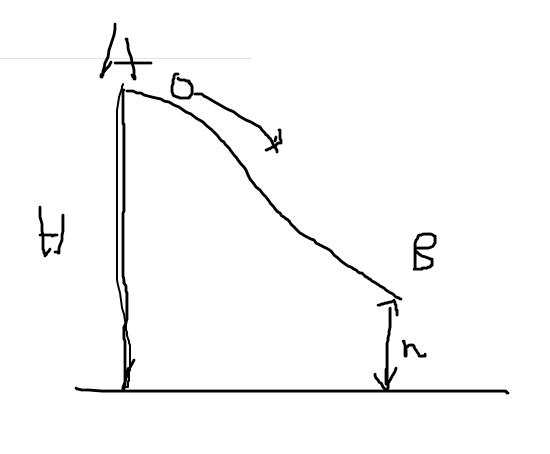
\includegraphics[width=0.3\textwidth]{vat.png}
    \caption{Hình bài 2}
    \label{vat}
\end{figure}
\subsection{Va chạm}
Trong phần này chúng ta sẽ khảo sát các bài toán liên quan đến va chạm đàn hồi và va chạm mềm
\subsubsection{Động lượng}
Động lượng của hạt được định nghĩa như sau: $$\vec{P}=m\vec{v}$$
Xét phương trình định luật II Newton, ta có:
$$\vec{F}=m\vec{a}=m\frac{d\vec{v}}{dt}=\frac{d \vec{P}}{dt}$$
Dễ thấy khi hệ hạt không có ngoại lực tác dụng thì $\vec{P}=const$, ta có định luật bảo toàn động lượng như sau: "Động lượng toàn phần của một hệ cô lập được bảo toàn". Chúng ta sẽ áp dụng định luật này để khảo sát hai bài toán va chạm thường gặp: va chạm đàn hồi và va chạm mềm
\subsubsection{Va chạm đàn hồi}
Va chạm đàn hồi là va chạm mà động năng của hệ trước và sau hệ được bảo toàn. Ở đây ta xét trường hợp hai quả cầu va chạm đàn hồi với nhau, quả cầu 1 di chuyển với vận tốc $v_{0}$ còn quả cầu 2 đứng yên.
\\Áp dụng định luật bảo toàn động lượng và động năng cho hệ vật, ta có:
$$\left\{\begin{array}{ll}
    m_{1}v_{0}=m_{1}v_{1}+m_{2}v_{2} &\\
    m_{1}v_{0}^2=m_{1}v_{1}^2+m_{2}v_{2}^2 &\\
    \end{array}\right.$$
Rút thế ta thu được:
$$\left\{\begin{array}{ll}
    v_{1}=\frac{m_{1}-m_{2}}{m_{1}+m_{2}}v_{0} &\\
    v_{2}=\frac{2m_{1}}{m_{1}+m_{2}}v_{0 } &\\
    \end{array}\right.$$
\subsubsection{Va chạm không đàn hồi}
Va chạm không đàn hồi là va chạm mà động năng của hệ trước và sau không được bảo toàn do có sự hao hụt năng lượng, ví dụ như khi ta thả một quả bóng xuống sàn, do có sự thất thoát năng lượng khi quả bóng va chạm vào mặt sàn nên nó không thể nảy cao lên độ cao ban đầu nữa. Ở đây chúng ta xét một trường hợp riêng của va chạm không đàn hồi, đó là va chạm mềm.
Va chạm mềm giữa hai quả cầu 1 và 2 được biểu diễn như hình vẽ, sau khi va chạm 2 quả cầu 1 và 2 dính vào nhau và chuyển động cùng một vận tốc V.
\begin{figure}
    \centering
    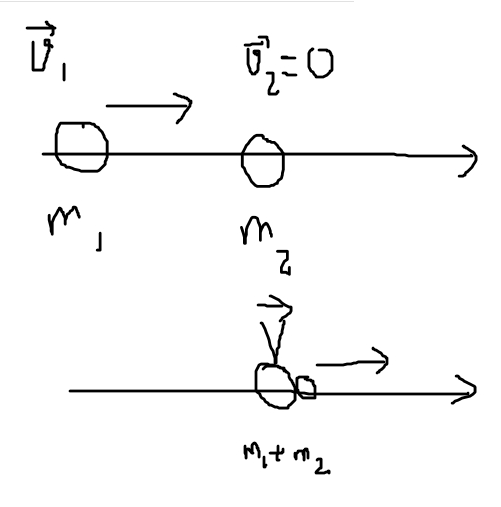
\includegraphics[width=0.5\textwidth]{mem.png}
    \caption{Va chạm mềm}
    \label{mem}
\end{figure}
Áp dụng định luật bảo toàn động lượng cho hệ vật, ta có $$m_{1}v_{1}=(m_{1}+m_{2})V$$
$$\Rightarrow V=\frac{m_{1}v_{1}}{m_{1}+m_{2}}$$
\\Ta tính được động năng của hệ vật trước và sau va chạm:
$$\left\{\begin{array}{ll}
    W_{d1}=\frac{m_{1}v_{1}^2}{2} &\\
    W_{d2}=\frac{m_{1}+m_{2}}{2}V^2=\frac{m_{1}^2v_{1}^2}{2(m_{1}+m_{2})} &\\
    \end{array}\right.$$
Phần động năng bị tiêu hao thành các dạng năng lượng khác (tỏa nhiệt hay năng lượng để liên kết 2 vật 1 và 2) là:
$$\Delta W_{d}=W_{d2}-W_{d1}=\frac{1}{2}m_{1}v_{1}^2\frac{m_{2}}{m_{1}+m_{2}}$$
Bài tập: Một viên đạn khối lượng m bay theo phương nằm ngang và đâm vào vật có khối lượng M được treo bởi 1 sợi dây có độ dài l như hình vẽ. Người ta thấy sợi dây bị lệch một góc $\alpha$ so với phương thẳng đứng. Hãy xác định vận tốc viên đạn trước khi đâm vào vật M và phần trăm động năng ban đầu của viên đạn chuyển thành nhiệt năng.
(Giả sử toàn bộ động năng sinh ra chỉ biến thành nhiệt năng)
\\Gợi ý: va chạm giữa viên đạn và vật M là va chạm mềm.
\begin{figure}
    \centering
    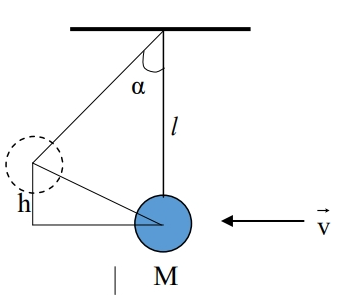
\includegraphics[width=0.5\textwidth]{dan.png}
    \caption{Hình minh họa}
    \label{dan}
\end{figure}
\section{Dao động và sóng cơ}
\subsection{Dao động}
Các công thức cơ bản cần nhớ:
\begin{tcolorbox}
    $$x=A\cos{(\omega t+\phi)}$$
    $$T=\frac{2\pi}{\omega}$$
    $$f=\frac{1}{T}$$
    $$v=x'=-A\omega\sin{(\omega t+\phi)}$$
    $$a=v'=-A\omega^2\cos{(\omega t+\phi)}=-\omega^2x$$
\end{tcolorbox}
\subsubsection{Con lắc lò xo}
Với con lắc lò xo thì:$$\omega=\sqrt{\frac{k}{m}}$$
Năng lượng của con lắc lò xo:
\begin{tcolorbox}
    $$W_{d}=\frac{1}{2}mv^2=\frac{1}{2}m\omega^2A^2\sin^2{(\omega t+\phi)}$$
    $$W_{t}=\frac{1}{2}kx^2=\frac{1}{2}m\omega^2A^2\cos^2{(\omega t+\phi)}$$
    $$W_{c}=\frac{1}{2}m\omega^2A^2$$
\end{tcolorbox}
\subsubsection{Con lắc đơn}
Với con lắc đơn thì: $$\omega=\sqrt{\frac{g}{l}}$$
Ta cũng có thể thiết lập các công thức tương tự.
\subsection{Sóng}
\subsubsection{Sóng ngang và sóng dọc}
\begin{itemize}
    \item Sóng ngang là sóng có phương truyền sóng vuông góc với phương dao động của các phần tử trong môi trường
    \item Sóng dọc là sóng có phương truyền sóng trùng với phương dao động của các phần tử trong môi trường
\end{itemize}
\begin{tcolorbox}
    $$\lambda=vT=\frac{v}{f}$$
Phương trình sóng tại điểm M cách gốc O một khoảng d là
$$u_{M}=a\cos{(\omega t-\frac{2\pi d}{\lambda})}$$
Phương trình giao thoa sóng tại điểm M cách nguồn A một khoảng $d_{1}$ và cách nguồn B một khoảng $d_{2}$ là:
$$u_{M}=a\cos(\omega t-\frac{2\pi d_{1}}{\lambda})+a\cos(\omega t-\frac{2\pi d_{2}}{\lambda})$$
\end{tcolorbox}
Tự biến đổi phương trình ở trên và suy ra các trường hợp đặc biệt.
\subsubsection{Sóng âm}
\begin{figure}
    \centering
    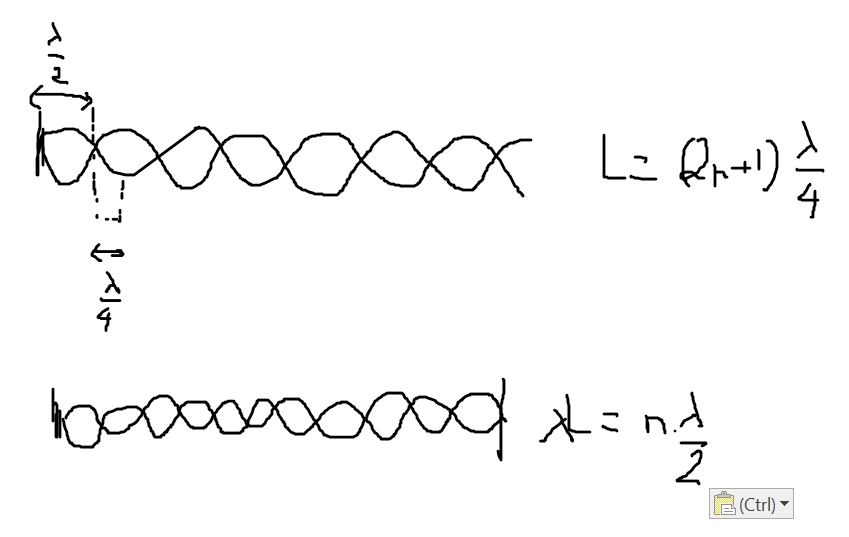
\includegraphics[width=0.5\textwidth]{song1.png}
    \caption{Sóng dừng với 1 đầu cố định và 1 đầu tự do}
    \label{song}
\end{figure}
Đây là hai công thức cần nhớ, sóng âm đã thi vào đề thi chính thức 1 lần.
\begin{tcolorbox}
    $$L=\log{\frac{I}{I_{0}}}$$ với $I_{0}=10^{-12}W/m^2$ là cường độ âm chuẩn
    $$P=\frac{I}{4\pi R^2}$$
\end{tcolorbox}
Bài tập: Một nguồn điểm phát ra sóng âm ở mọi hướng trong không gian với công suất trung bình 100W. Hãy xác định:
\begin{enumerate}
    \item Cường độ âm tại khoảng cách 5m tính từ nguồn
    \item Mức cường độ âm tại điểm đó
\end{enumerate}
